\appendix
\section{Standard di qualità}
	\subsection{ISO/IEC/IEE 12207:2017}
	ISO/IEC/IEE 12207 è uno standard che descrive un insieme di processi utilizzabili nel ciclo di vita del software. 
	Sebbene promuova la qualità nello sviluppo del software, lo standard permette totale libertà sulla scelta di un modello del ciclo di vita e dei processi che lo compongono. Ogni gruppo può quindi scegliere di usare i processi forniti e adattarli alle proprie esigenze, o addirittura crearne di nuovi.\newline 
	Nel documento è anche presente un glossario di termini, definizioni e abbreviazioni che è un ottimo punto di partenza per avvicinarsi al linguaggio tecnico.\newline 
	I processi sono stati determinati seguendo questi criteri:
	\begin{itemize}
		\item un processo interconnette attività, task\glosp e risultati;
		\item i processi sono tra loro il più possibile indipendenti;
		\item un processo dev'essere attuabile da una singola organizzazione (nella fattispecie dal nostro gruppo).
	\end{itemize}
	Ogni processo è organizzato seguendo le seguenti voci:
	\begin{itemize}
		\item nome descrittivo;
		\item scopo;
		\item risultati attesi;
		\item attività
		\item task;
	\end{itemize}
	Infine, i processi sono raggruppati in quattro gruppi.
		\subsubsection{Processi di Accordo}
		Gli accordi sono la modalità secondo cui due organizzazioni comunicano per la compravendita di un prodotto software. Una di queste, che commissiona il software che intende comprare, ha il ruolo di acquirente, mentre l'altra, che fornisce il software richiesto, è il fornitore. Entrambe le organizzazioni riescono a ottenere valore, l'una dall'acquisto di uno strumento utile, l'altra dal lavoro svolto per realizzarlo.
		I processi in questione sono di carattere organizzativo, ma stanno al di fuori del ciclo del software, costituendo quindi una categoria separata dagli organizzativi.
		\subsubsection{Processi Organizzativi \textit{project-enabling}}
		Appartengono all'organizzazione e operano a un livello più alto rispetto ai progetti, ai quali non sono circoscritti. Sono fatti per creare un'ambiente all'interno del quale i progetti possono essere sviluppati. Essi riguardano il modello del ciclo di vita del software, la gestione del team e della qualità. Tutti insieme rappresentano l'immagine dell'azienda, visibile da chi non ne fa parte.
		
		\begin{figure}
			\centering
			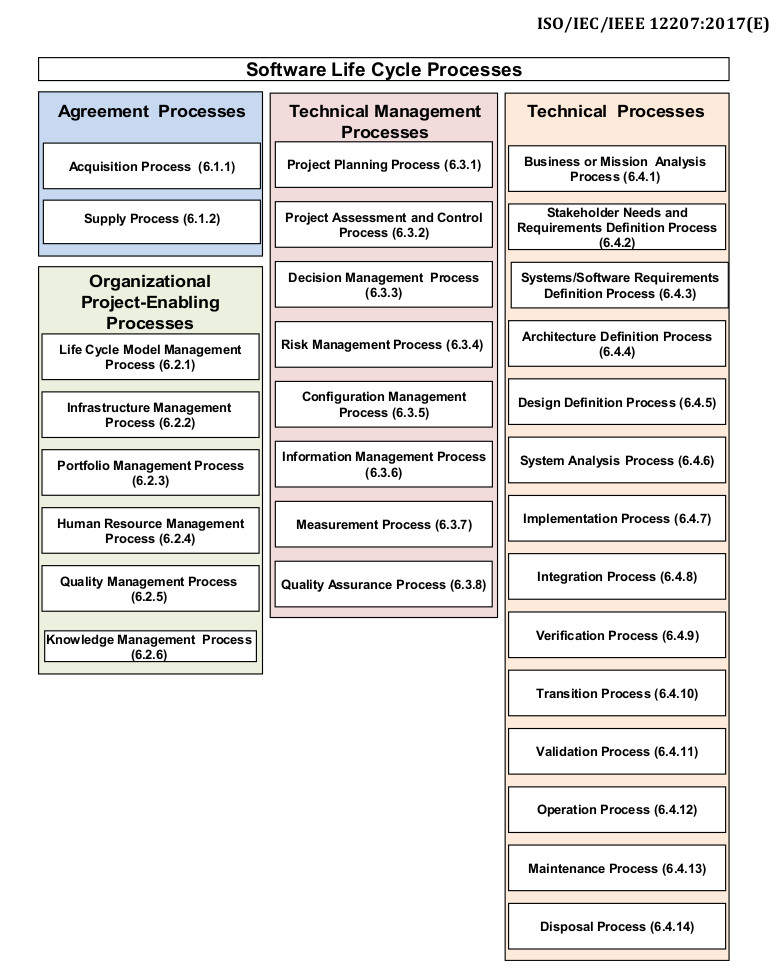
\includegraphics[scale=0.5]{res/images/software_life_cycle_processes.jpg}\caption{Processi del ciclo di vita del software}	
		\end{figure}
	
		\subsubsection{Processi di Gestione Tecnica}
		I processi di gestione tecnica fanno uso delle risorse a disposizione per adempiere agli obblighi contrattuali. Alcuni di questi riguardano:
		\begin{itemize}
			\item la pianificazione in termini di tempi, costi e obiettivi;
			\item le azioni di controllo per aderire ai piani di progetto e di qualifica;
			\item le informazioni e le loro modalità di produzione, aggiornamento, distribuzione e archiviazione;
			\item in generale, le strategie e le azioni a supporto dei processi tecnici.
		\end{itemize}
		
		\subsubsection{Processi Tecnici}
		I processi tecnici riguardano la trasformazione delle richieste degli stakeholder nel prodotto concreto, che ha la forma di un sistema software.
		
		
			
	
	\pagebreak
	\subsection{ISO/IEC 9126}
	ISO/IEC 9126 è uno standard internazionale per valutare la qualità del software.\\%PLACEHOLDER mettere eventuale immagine dello standard
	Questo standard è diviso in quattro parti:
	\begin{itemize}
		\item \textbf{Modello della qualità del software} (descritto dopo le successive 3 parti)
		\item \textbf{Metriche per la qualità interna}:metriche che si applicano al software non eseguibile durante le fasi di progettazione e codifica. Permettono di individuare eventuali problemi che potrebbero influire sulla qualità finale del prodotto prima che venga realizzato un eseguibile. Grazie alle misure effettuate tramite le metriche interne è possibile prevedere il livello di qualità esterna e di qualità in uso del prodotto finale, poiché entrambe vengono influenzate dalla qualità interna.\\
Viene rilevata tramite analisi statica. Idealmente la qualità interna determina la qualità esterna;
		\item \textbf{Metriche per la qualità esterna}: metriche applicabili al software in esecuzione che ne misurano il comportamento attraverso dei test, in funzione degli obiettivi stabiliti.\\
Viene rilevata tramite analisi dinamica. Idealmente la qualità esterna determina la qualità in uso;
		\item \textbf{Metriche per la qualità in uso}: metriche applicabili solo al prodotto finito ed in uso in condizioni reali.\\
La qualità in uso viene raggiunta solo se è stato raggiunto il livello di qualità interna e di qualità esterna.
	\end{itemize}
	Il modello di qualità del software, presentato nella prima parte dello standard, suddivide la qualità in sei caratteristiche generali e varie sotto caratteristiche, misurabili attraverso delle metriche, utilizzate per fornire una scala ed un metodo per la misurazione. Ecco l'elenco delle caratteristiche:
	\begin{itemize}
		\item \textbf{Funzionalità}: capacità del software di soddisfare i requisiti, descritti nell'Analisi dei Requisiti, in un determinato contesto.\\
Nello specifico il software deve soddisfare le seguenti caratteristiche:
		\begin{itemize}
			\item \textbf{Appropriatezza}: capacità di fornire funzioni appropriate per attività specifiche, che permettano di raggiungere gli obiettivi prefissati;
			\item \textbf{Accuratezza}: capacità di fornire i risultati concordati o la precisione richiesta;
			\item \textbf{Interoperabilità}: capacità di interagire ed operare con uno o più sistemi specificati;
			\item \textbf{Conformità}: capacità di aderire a standard;
			\item \textbf{Sicurezza}: capacità di proteggere informazioni e dati.
		\end{itemize}
\item \textbf{Affidabilità}: capacità del software di mantenere uno specifico livello di prestazioni quando usato in condizioni specificate.\\
Nello specifico il software deve soddisfare le seguenti caratteristiche:
		\begin{itemize}
			\item \textbf{Maturità}: capacità di evitare il verificarsi di errori, malfunzionamenti o risultati non corretti;
			\item \textbf{Tolleranza agli errori}: capacità di mantenere livelli prefissati di prestazioni anche in presenza di malfunzionamenti o usi scorretti del prodotto finale;
			\item \textbf{Recuperabilità}: capacità di ripristinare un livello appropriato di prestazioni o di recupero di informazioni rilevanti a seguito di un malfunzionamento;
			\item \textbf{Aderenza}:  capacità di aderire a standard, regole e convenzioni che riguardano l'affidabilità.
		\end{itemize}
\item \textbf{Efficienza}: capacità del prodotto software di eseguire le proprie funzioni minimizzando il tempo necessario e sfruttando al meglio le risorse che necessita.\\
Nello specifico il software deve soddisfare le seguenti caratteristiche:
		\begin{itemize}
			\item \textbf{Nel tempo}: capacità di fornire adeguati tempi di risposta, elaborazione e velocità di attraversamento in determinate condizioni;
			\item \textbf{Nello spazio}: capacità di utilizzo di quantità e tipo di risorse in maniera adeguata;
		\end{itemize}
\item \textbf{Usabilità}: capacità del prodotto software di essere compreso, appreso, usato e accettato dall'utente, quando usato sotto determinate condizioni.\\
Nello specifico il software deve soddisfare le seguenti caratteristiche:
		\begin{itemize}
			\item \textbf{Comprensibilità}: capacità di essere chiaro riguardo le proprie funzionalità e il proprio utilizzo;
			\item \textbf{Apprendibilità}: capacità di essere facilmente apprendibile dagli utenti;
			\item \textbf{Operabilità}: capacità di permettere all'utente di eseguire i suoi scopi e controllarne l'uso;
			\item \textbf{Attrattività}: capacità di essere piacevole all'utente che l'utilizza.
		\end{itemize}
\item \textbf{Manutenibilità}: capacità del software di essere modificato, al fine di aggiungere correzioni, miglioramenti o adattamenti.\\
Nello specifico il software deve soddisfare le seguenti caratteristiche:
		\begin{itemize}
			\item \textbf{Analizzabilità}: capacità di essere facilmente analizzato al fine di localizzare un errore;
			\item \textbf{Modificabilità}: capacità di poter essere agevolmente modificato nel codice, nella progettazione o nella documentazione;
			\item \textbf{Stabilità}: capacità di evitare effetti indesiderati a seguito di una modifica;
			\item \textbf{Testabilità}: capacità di essere facilmente testato per validare le modifiche apportate.
		\end{itemize}
\item \textbf{Portabilità}: capacità del software di essere trasportato da un ambiente di lavoro ad un altro, sia esso hardware che software.\\
Nello specifico il software deve soddisfare le seguenti caratteristiche:
		\begin{itemize}
			\item \textbf{Adattabilità}: capacità di essere facilmente adattato a differenti ambienti operativi, senza applicare modifiche;
			\item \textbf{Installabilità}: capacità di poter essere installato in un determinato ambiente;
			\item \textbf{Conformità}: capacità di coesistere con altre applicazioni e di condividere risorse;
			\item \textbf{Sostituibilità}: capacità di essere utilizzato al posto di un altro software per svolgere gli stessi compiti, nello stesso ambiente.
		\end{itemize}
	\end{itemize}
